\chapter{Atmosphäre and Instrumente}\label{cha:atmosph}
\xc bietet ein internes Modell der Athmosphäre welches auf statistischen Daten beruht,
welche während des Fluges durch die angeschlossenen Sensoren empfangen wurden.

Diese statistischen Daten sind alle lediglich Annahmen und Vorhersagen und können -wie wir alle
aus Erfahrung gut wissen-  sich innerhalb sehr kurzer Zeit stark ändern.

Daher sollte man sich nicht zu sehr auf die Vorhersagen der Geräte und internen Routinen verlassen.
Es ist immer ein gesundes maß an Mißtrauen angesagt, eine permanente, gute Wetterbeobachtung
ist grundsätzlich angebracht. Speziell bei kritischen Situationen wie z.B.\ auch
Außenlandungen sollten die Augen immer draußen sein, und nicht zu sehr auf die Instrumente
gerichtet sein.
\section{Variometer}
\subsection*{Analog- Variometer}\index{Vario!Analoganzeige}
Die Anzeige des Variometers als Analoganzeige ist aus Platzgründen nur im Querformat möglich.

Das Variometer \textsl{kann} als animiertes Zeigerinstrument dargestellt werden.
Das Bruttovaro stellt die berechneten Steig- und Sinkwerte sowohl in als Zeiger als
auch in Textform in der Mitte der Anzeige dar.

Zusätzlich können Sollfahrtpfeile über bzw. unter der Brutto Vario Anzeige erscheinen,
welche die Sollfahrt angeben. Nach unten zeigende Pfeile bedeuten: ''schneller'', nach oben
gerichtete Pfeile heißen ''langsamer'' fliegen.

Im Kurbelmodus zeigt der Integrator das über die letzten 30 Sekunden ermittelte Bruttosteigen als Mittelwert.
Im Vorflugmodus dagegen zeigt der Integrator das über die letzten 30 Sekunden ermittelte Nettosteigen der Luftmasse an.
\marginpar{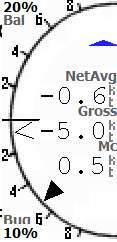
\includegraphics[angle=0,width=0.5\linewidth,keepaspectratio='true']{figures/gaugevario2.png}}

Der Integrator kann optional ebenfalls dargestellt werden - er erscheint dann als Diamant am Rande der Skala.
Die Vario Anzeige ist komplett varierbar \config{variogauge}, so daß alle Zeiger und Werte einzeln dargestellt
werden können. 

\subsection*{Digitales Variometer}\index{Vario!Digitalanzeige}
Es besteht die Möglichkeit, das Vario nicht ausschließlich als Analoganzeige innerhalb der
\menulabel{\bmenut{Konfig.}{2/3}\blink\bmenus{System}}Infoboxen darstellen zulassen,
sondern in der Art, wie auch die Endanflughöhe dargestellt wird.


Mit \button{Vario Bar} kann dies Verhalten ein- bzw. ausgeschaltet werden.

\menulabel{\button{Anzeigen}\blink\button{Flarm etc.}}
Hierzu werden am rechten Rand des Bildschirmes auf gleicher Höhe mit dem Endanflughöhenanzeiger
Pfeile nach oben in grün für Steigen, und Pfeile in rot nach unten für Saufen angezeigt.
Ein zusätzlicher grauer Teilpfeil zeigt entsprechend der Skalierung den aktuellen MC-Wert an.

Die Skalierung der Pfeile sind 5m/sec. Werte über 5m/sec werden durch die abgesetzte Peilspitzenangegeben. 
\sketch{figures/vario-bar.png}
Der hellgrüne/hellrote  Pfeil zeigt das integrierte Steigen/Saufen  an, so kann man mit einem Blick erkennen, wie gut der MC-Wert (der ja grau hinterlegt ist) gewählt ist. Ist der hellgrüne Pfeil auf gleicher Höhe mit dem MC-Peil, hat man sehr gut gewählt.

Die Zahl im  Textfenster gibt zusätzlich das integrierte Steigen der letzten 30 Sekunden an.

\warning Eine Sollfahrtanzeige  ist bislang nicht vorgesehen.



Wenn ein intelligentes Vario angeschlossen ist, dann werden die Werte direkt vom Vario an den Zeiger
übertragen, es entfallen die \xc-Routinen zur Berechnung. Andernfalls stellt  \xc die Werte basierend aus
übermittelten GPS und barometrischen Drucksondenwerten z.B.\ vom \fl dar. Diese Werte sind natürlich wesentlich
langsamer und vor allem unkompensiert.

MacCready Wert, Mücken und Ballast Sollfahrt sowie Wind werden zwischen  \xc und einem
intelligenten Vario ausgetauscht. Idealerweise können in einem solchen Zusammenspiel beide Instrumente (\xc und das intelligente Vario) auf alle Daten zurückgreifen, so daß Mehrfachbedienungen nicht mehr notwendig sind.
(Will heißen: Eine Eingabe z.B.\ des MC-Wertes in  \xc wird auch vom int.\ Vario benutzt und umgekehrt)

Eine Liste der unterstützten Varios kann in Kapitel  ~\ref{sec:supported-varios} nachgesehen werden.

Bei Verwendung des \textsf{Vega}, wird ein kleines kreisendes Segelflugzeug dargestellt, wenn sich das Vario
im Kurbelmodus befindet.
\section{Datenerfassung der Luftmasse}%Air data inputs}

Wenn extern erfaßte Werte der Luft (Geschwindigkeit, Höhe etc.) von angeschlossenen Geräten zur Verfügung
stehen, kann und wird \xc diese für interne Berechnungen und Anzeige in InfoBoxen benutzen.
Selbstverständlich sind diese Berechnungen erheblich genauer und schneller als allein über das GPS
erfaßten Singale.

Die wichtigsten von  \xc benutzen Daten sind:
\begin{description}
\item[\textit{Totalenergie Vario}]
(Änderung der Totaleneergie der durchflogenen Luftmasse)
Benutzt für die Anzeige und für die Berechnung des Nettosteigens
\item[\textit{Netto Variometer}]
(ermitteltes Steigen der durchflogenen Luftmasse)
Wird benutzt für die Anzeige und um den Flugweg auf der Karte darzustellen.
Erlaubt so effektiv eine Darstellung von Steig- uns Sinkpfaden
\item[\textit{Beschleunigung des Flugzeuges}]
(g-Wert) Benutzt für die Berechnung des Netto Variometers, falls externe Sensoren (Varios) nicht angeschlossen sind.
\item[\textit{Barometrische Höhe}] Wird benutzt für die Anzeige
\item[\textit{IAS Angezeigte Luftgeschwindigkeit}]
Benutzt für die Anzeige, zur Kompensation der kinetischen Energie während des Endanfluges  und im Nettovariometer,
sofern keine externe Variosignale vorhanden sind.
\item[\textit{Luftdichte}] Benutzt für die Berechnung der wahren Geschwindigkeit (TAS) aus der angezeigten Geschwindigkeit (IAS)
\end{description}
\section{Windanzeige}
Windrichtung und -stärke werden kontinuierlich auf der Karte dargestellt.
Die Länge des Pfeiles steht für die Stärke des Windes, eine Textdarstellung erfolgt
ebenfalls in unmittelbarer Nähe der Pfeilspitze.

Die Berechnung erfolgt über die Abdrift des Flugzeuges während des Kurbelns (im Kurbelmodus), s. Kap.~ \ref{sec:wind-estimation}.
\marginpar{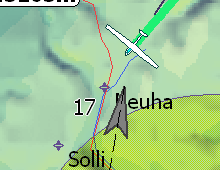
\includegraphics[angle=0,width=0.5\linewidth,keepaspectratio='true']{figures/wind-arrow.png}}
Optional können diese Werte in Infoboxen dargestellt werden.

Die Winddaten sind neben anderen sehr wichtig für die Berechnung des Endanfluges.
Es ist daher möglich, die Winddaten manuell zu korrigieren.

\section{Wind Ermittlung}\label{sec:wind-estimation}
\xc bietet zwei verschieden Wege, den Wind während des Fluges zu ermitteln.
\begin{description}
\item[\textit{Beim Kurbeln}]  Diese Methode benutzt die  GPS Koordinaten um die Abdrift während
des Kurbelns zu ermitteln und ist bei allen \xc Installationen verfügbar, da unabhängig von anderen Sensoren.
\item[\textit{ZickZack Flug}] Diese Methode benutzt sowohl die GPS Daten wie auch die Werte aus der TAS-Messung.
Dies ist nur verfügbar, wenn \xc an ein inelligentes Variometer mit entsprechendem Ausgang angeschlossen ist.
\end{description}

Da die Winddaten während des Kurbelns erfaßt werden, liegen diese als Mittelwert über der erkurbelten Höhe und
zu unterschiedlichen Zeiten vor. Wenn sich die Höhe des Flugzeuges signifikant ändert wird daher aus den
bisher gesammelten Werten ein Optimum errechnet.

Bei der PC und Pocket-PC-Version mit Touch-Screen kann auch mittels der Wind-InfoBox der Wind in
üblicher Weise geändert werden:
Längeres Tippen auf die InfoBox (Windrichtung bzw.\ -geschwindigkeit) läßt eine Auswahlbox
erscheinen, auf der die Werte angepaßt  werden können.

Über das Feld ''Auto Wind'' in den Konfigurationseinstellungen \config{autowind} kann
eingestellt werden, welcher der Routinen benutzt werden soll

\begin{itemize}
\item Manuelll
\item Kurbeln
\item ZickZack
\item Beides (ZickZack und Kurbeln)
\end{itemize}

Wenn sich Windrichtung und/oder -stärke ändern, erscheint eine Meldung  auf dem Bildschirm begleitet von einem Ton.
\subsection*{Kurbel--Algorythmus der Windermittlung}
\xc ermittelt Windstärke und -richtung während des Kurbelns. Dies geschieht über einen ausgefeilten Algorythmus, welcher den Versatz über Grund während eines ganzen kreises im Bart ermittelt. Ovales Kurbeln mit ständig ändernder Querneigung vermindern die Qualität der Berechnung ganz beträchtlich, da dann der Flugweg extrapoliert werden muß. Die besten ergebnisse gibt es, wenn wirklich kreisrund mit konstanter Querneigung geflogen wird.\index{Wind!Ermittlung}

Die Berechnung kann nur erfolgen wenn die GPS-Quelle mehr als einen Fix pro zwei Sekunden ausgibt. 
Da --aus Erfahrung-- immer mit GPS-Ausfällen gerechnte werden muß, wurde dies als Mindestanforderung zur halbwegs glaubwürdigen Windermittluing vorausgesetzt.  
 
\subsection*{ZickZack--Algorythmus}
Für Flugzeuge, welche mit einem intelligenten Variometer ausgestattet sind, welches
an \xc angeschlossen ist, bietet \xc die Möglichkeit, des ZickZack Algorythmus
zur Ermittlung der Windkomponente.

Mit dieser Methode ist es möglich, den Wind in Stärke und Richtung zu ermitteln, ohne Kurbeln zu müssen.
Dies erlaubt es dem Piloten,  während des Vorlfiegens den Wind z u ermitteln, wobei lediglich ein
bißchen ''ZickZack'' geflogen werden muß.

Es ist nicht unbedingt ein spezielles Manöver zu fliegen, denn normalerweise  fliegt der Pilot auf
der Suche nach Thermik immer etwas nach links und nach rechts. Normalerweise benötigt diese
Methode ein Abweichen vom Kurs von ca. 40$^\circ$.

Wenn sich der Wind im Geradeausflug erheblich ändert wird der ZickZack-Algorythmus dazu benutzt
um den Wind zu aktualisieren - auch dann wenn sich der Kurs des Flugzeuges kaum oder nur wenig ändert.
Höhere genauigkeiten sind damit erzielbar.

Die Windermittlungen werden grundsätzlich aktualisiert, wenn sich größere Änderungen zwischen  der
ermittelten Grundgeschwindigkeit und der wahren Grundgeschwindigkeit (z.B. GPS)
im Geradeausflug entdeckt wurden.
\subsection*{Kompaß - Algorythmus}
Für Flugzeuge, die mit einem intelligenten Variometer und einem Kompaßabgriff der
Windrichtung ausgestattet sind, ermöglicht  \xc die Benutzung dieser Werte direkt.
Hierdurch ist es überflüssig, für die Windermittlung zu kurbeln oder zickZack zu fliegen.
\section{Windeinstellung}\index{Wind!Einstellung}\label{sec:Windeinstellung}
Der Wind-Dialog gestattet die einmalige Grundeinstellung der Werte  z.B.\ am Boden und\menulabel{\bmenut{Konfig}{1/3}\blink\bmenus{Wind}}
anschließende Aktualisierung bei Bedarf in der Luft. 

Wenn der Dialog geschlossen wird, werden die ermittelten Werte solange benutzt,
 bis neue Werte aus der ZickZack- oder Kurbelmessung vorliegen.

Der automatische Windalgorythmus kann auch abgeschaltet oder aber es können
beide Methoden verwandt werden (s.o. Bild) Siehe Kap.~\ref{sec:wind-estimation}
\sketch{figures/dialog-wind2.png}zu den Details dieser Algorythmen.

Die Windabdrift in der Darstellung des geflogenen Pfades  auf der Karte kann ebenso an-
oder ausgeschaltet werden. Nähere Details hierzu in Kap.~\ref{sec:trail}.
\section{Thermikprofil}\index{Thermikprofil}
Um das beste Höhenband schnell ausfindig zu machen, werden Daten über die Steigwerte in
Abhängigkeit von der geflogenen Höhe aufgenommen.
Diese Anzeige wird auf der linken Seite der Karte oberhalb der Endanflugshöhenindikatoren dargestellt.
Sie ist nicht sichtbar, wenn man sich oberhalb des Gleitpfades befindet.

Das Thermikprofil ist horizontal skaliert gemäß des bislang besten mittleren Steigens.
Vertikal wird die Höhe dargestellt und skaliert gemäß der höchsten bislang erreichten Höhe nach dem Start
\marginpar{\hbox{\vbox{\centering{ 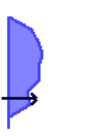
\includegraphics[angle=0,width=0.5\linewidth,keepaspectratio='true']{figures/thermalprofile.png}}}}}
(Siehe hierzu Kap.~\ref{sec:safety-heights}). Ein schwarzer Pfeil gibt die derzeitige Höhe des Flugzeuges an.
Die Länge des  Pfeil ist nach dem derzeit eingestellten MC-Wert skaliert und gibt somit eine schnellstmögliche Übersicht über die Qualität und evtl. Abweichung des aktuellen MC-Wertes innerhalb des durchflogenen Höhenbandes.

Wenn sich der Pilot auf Thermiksuche befindet kann somit die Position des Pfeiles ein Anhaltspunkt sein,
wie wichtig es ist, wieder Thermik zu finden\dots
Wenn der Pfeil sich auf den unteren Rand des Bandes zubewegt, befindet sich das Flugzeug nahe der Aufbruchshöhe und der Pilot sollte sich allmählig damit abfinden, nun auch in schwächerer Thermik kurbeln zu müssen.

\section{Thermikfinder}
Durch einen Algorythmus wird der Kern der Thermik errechnet und dargestellt.
Das Symbol für das Zentrum ist eine kleine grüne Spirale auf der Karte der moving map.
\sketch{figures/shot-tlocator-circling.png}
Der Thermikfinder markiert \textit{fortlaufend  die letzten 20 Bärte} während des Fluges auf der Karte.
Die Position des Zentrum kann mit der Abdrift durch den ermittelten Wind korrigiert werden.

Dies bedeutet, daß \xc sich die Position der Thermikquelle intern über Grund merkt.
Mit anderen Worten, wenn Du einen Bart ganz oben verläßt, und später zu diesem in tieferen
Höhen zurückkehrst wird die angezeigte Position auf der Karte die Position in der
entsprechenden Höhe sein (welche etwas luvwärts stehen wird als die Basis.)
\sketch{figures/shot-tlocator-cruise.png}

Wenn sich der Wind ändert und die Thermikquelle noch immer aktiv ist,
wird die Position auf der Karte ein Hinweis für die Windänderung sein, denn
durch die Abdrift in der Höhe ist der Bart mit dem Wind gewandert.

\section{Zentrierhilfe (info info Zentrierhilfe)}\index{Zentrierhilfe}
Die Zentrierhilfe ist eine graphische Hilfe, um den Kern der Thermik zu treffen und einfach zu zentrieren.
Wenn diese in den Konfigurationseinstellungen aktiviert ist ( \config{thermalassistant}), erscheint beim
Kurbeln wodurch ein kleines  rundes Diagramm. Ein kurzer Tip auf dies Diagramm läßt die Zentrierhilfe im Vollbild erscheinen.

Die Polardarstellung zeigt die Steigrate über den kreisförmig en Kurs des Flugzeuges an.
Die Photos hier zeigen das Flugzeug beim Rechtskurbeln, während das Flugzeug an der linken
Seite des Diagrammes fixiert ist und die Verteilung der Steigwerte vom Zentrum zum Rande hin zunehmen.

Je "runder" man zentriert hat, desto kreisförmiger wird das Diagramm. Ideal wäre eine kreisrunde
Darstellung, was bedeutet, das das Steigen auf dem ganzen Kreis identisch ist.

\begin{tabular}{c c}
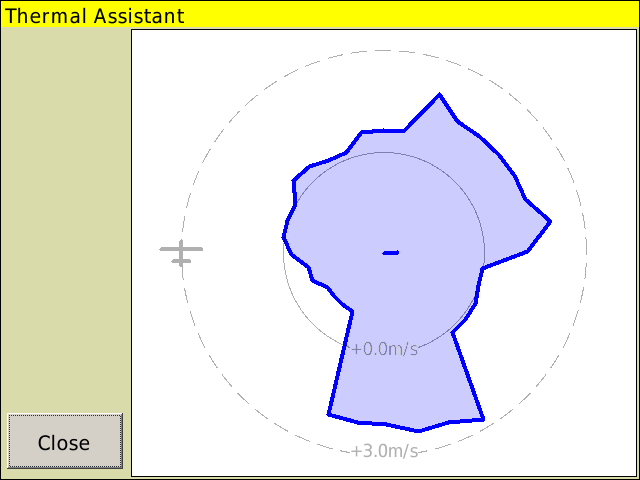
\includegraphics[angle=0,width=0.5\linewidth,keepaspectratio='true']{figures/dialog-thermal-assistant0.png}&
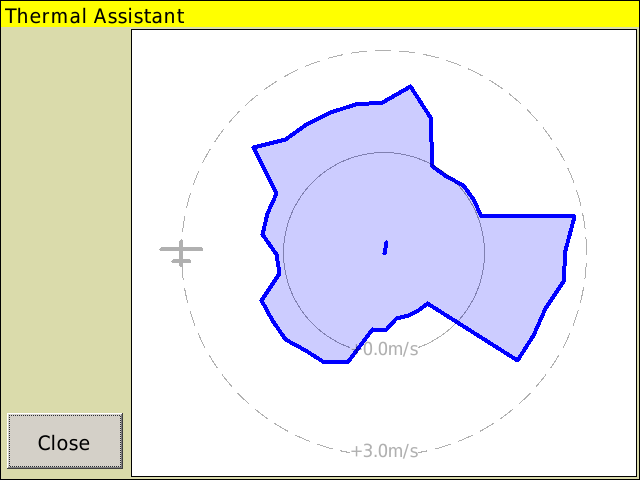
\includegraphics[angle=0,width=0.5\linewidth,keepaspectratio='true']{figures/dialog-thermal-assistant1.png}\\
\end{tabular}

Die Photos sind wenige Sekunden nacheinander aufgenommen worden um zu zeigen, wie mit der Zentrierhilfe
in  der Praxis umgegangen  werden kann. Ein ganz einfaches Rezept zum Umgang hiermit ist hier in zwei Schritten aufgezeigt:

\begin{description}\index{Zentrierhilfe!Umgang}
\item[1.]  In dem Moment, wo das Maximum des Steigens  (die ''Beule''\dots) am  oberen Rand des Diagrammes  vorbeigeht
(das ist ca. ein Viertelkries bevor Du diese Stelle mit Deinem Flugzeug wieder erreichen wirst) öffnen den
Kreis ein wenig durch Flacher werden um so dem Zentrum des Steigens näher zu kommen.
\item[2.]  In dem Moment wo das maximale Steigen an Deinem abgebildeten Flugzeug vorbeikommt,
sollte das Vario das maximale Steigen anzeigen. Jetzt wieder enger werden (sehr eng), um in das
beste Steigen einzusteigen.
\end{description}

Es muß hierbei ausdrücklich gesagt werden, daß die Qualität dieses Verfahrens auch sehr von der
angeschlossen
Hardware (externe Sensoren,  Leistungsfähigkeit des PDA o.ä.) abhängt. Durch die Verzögerung der
Signale kann es sein, daß vorher oder später ein und wieder ausgeleitet werden muß.
Ein bißchen Training mit diesem Verfahren um  erfolgreich zu zentrieren ist sicher unumgänglich.


\section{Konvektionsvorhersagen}\label{sec:convection-forecast}\index{Konvektionsvorhersage}
Wenn das Flugzeug mit einem Außentemperatur- und Feuchtefühler ausgestattet ist, kann anhand
\menulabel{\bmenut{Konfig}{1/3}\blink\bmenus{Flug}}vorhandener und ermittelter Daten  eine simple Vorhersage der Basishöhe und Konvektion vorgenommen werden. Der Feuchtesensor wird vorwiegend für die Ermittlung der Basishöhe benutzt.

Hierzu muß der Pilot vor dem Flug die maximal erwartete Temperatur in einer Infobox eingeben.
 Siehe Kap.~\ref{sec:basic-sett-dial}.

Die vorhergesagte  Untergrenze der der konvektiven Schicht (d.h. der für Segelflieger i.d.R.\ interessante
Bereich der Athmosphäre) wird angenommen, als die Schicht, in der Temperatur der Athmosphäre gleich der maximalen vorhergesagten Bodentemperatur ist, (trockenadiabtische Abkühlung angenommen).
Wenn die Athmosphäre stabil ist, wird die Konvektionsbasis als Null angegeben.

Die vorhergesagte Basis der Wolken wird bestimmt von der Höhe, in welcher der Taupunkt die
maximal vorhergesagte Bodentemperatur erreicht, wobei sich das Luftpaket sich trockenadiabatisch bis
zu der Höhe abkühlt, wo es die Feuchtadiabate schneidet. Wenn keine Wolken vorhergesagt werden, wird die Basis als Null ausgegeben.

\section{Analyse - Dialog}\index{Analyse}
Dieser Dialog kann für verschiedene Kontrollfunktionen bzw.\ Informationen benutzt werden 

\menulabel{\bmenus{Info}\blink\bmenus{Analyse}}


Folgende Seiten das Wetter betreffend sind hier enthalten:
\begin{description}
\item[Wind über Höhe]
Zeigt die Windgeschwindigkeit und Richtung über die Höhe an.

Der Button \button{Wind einstellen} öffnet die Windeinstellung, z.B.\ um Wind manuell zu korrigieren.

\item[Temperaturverlauf]
\sketch{figures/analysis-wind.png} Diese Seite ist nur verfügbar bzw.\ mit Daten gefüllt, wenn ein entsprechendes Instrumentan  \xc angeschlossen ist, welches die Außentemperatur und Feuchtigkeit angibt.

Das Diagramm zeigt den Verlauf von Temperatur der trockenen Luft, Taupunkt, und Außentemperatur
über der Höhe. Weiterhin wird die hieraus ermittelte Wolkenbasis und die Konvektionshöhe  angegeben.


\end{description}
Das Barogramm (Kap.~\ref{sec:analysis-dialog-climb}) und der Verlauf des Steigens über der Höhe sind
ebenfalls in diesem Dialog zu finden, werden jedoch an anderer Stelle beschreiben.
\sketch{figures/analysis-temptrace.png}

\section{Wettervorhersage, RASP}\index{Wettervorhersage}
Es können Wettervorhersagen, welche auf den RASP-Berechnungen (Regional Atmospheric
Soaring Prediction) basieren als Karte anstelle \menulabel{\bmenut{Info}{2/3}\blink\bmenus{Wetter}}der Darstellung des Geländes eingeblendet werden. \\

Dazu muss natürlich die Gelände Anzeige eingeschaltet sein. \tip{} \\

Des weiteren muß ein für den entsprechenden Flugtag gültiges File \verb"xcsoar-rasp.dat"  in
das \xc - Verzeichnis kopiert werden, auf das  \xc zugreifen kann.

In diesem Abschnitt soll nur auf die Anwendung eingegangen werden; eine ausführliche
Beschreibung der Details von RASP gibt es in  \url{www.drjack.info}.
und welche Limitierungen diese Art von Vorhersage innehat.

Die einzelnen Arten der Überlagerung auf der Karte (z.B.\ Basishöhe, Niederschlag,
max.\ Temperatur etc.\  können dort aufgerufen werden.
Die einzelnen Parameter werden unten erklärt und sind auch im Feld \button{Hilfe} zu finden.

In der Auswahlbox kann der gewünschte darzustellende Wert angeklickt werden.
Die Vorhersagezeit kann eingestellt werden. Felder bzw.\ Werte, in RASP derzeit nicht verfügbar sind,
haben einen leeren Hintergrund.

 Wenn \button{Zeit}  angewählt wird, wird die Vorhersage auf die nächst mögliche im RASP-File
enthaltene Zeit bestimmt. \sketch{figures/dialog-weather.png} Derzeit gibt es nur eine Auswahl: ''Sofort"

Name, Maximal und Minimalwert (z.B.\ Temperatur) sind in den jeweiligen Karten enthalten.
Der Name der Karte ist am Rande unten links der Karte gezeigt.

Folgende Karten sind über das  \button{Feld} bislang anwählbar:
\begin{description}
\item[Gelände] Zeigt die normale Geländekarte ohne Wetterdaten
\item[W*]
Mittleres Steigen  der trockenen Thermik in Bereich der mittleren Konvektionsschicht.
Abzüglich des Eigensinkens erhält man in die Varioanzeige  bei Blauthermik.

Bei Wolkenthermik können die Bärte stärker sein als diese Vorhersage,  da die
Kondensation zusätzlich Aufwinde generiert.

Der ''Wolkensog''  wird hierbei vernachlässigt.
W$^\ast$ hängt von der Erwärmung des Bodens  und von der Dicke der Konvektionsschicht ab.

\begin{center}
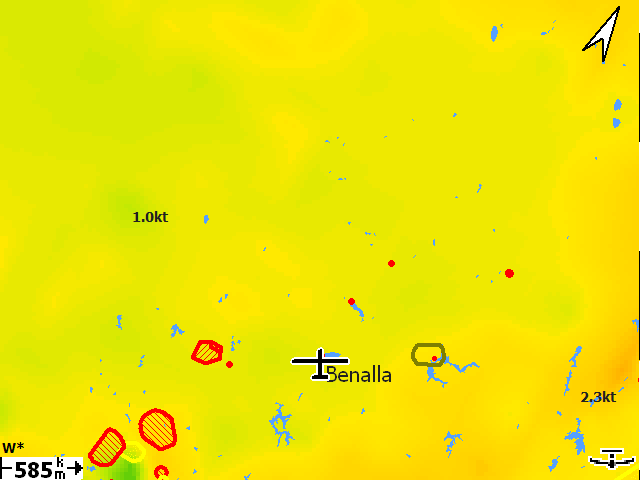
\includegraphics[angle=0,width=0.8\linewidth,keepaspectratio='true']{figures/rasp-wstar.png}
\end{center}

\item[KS WindGschw]
Stärke und Richtung des gemittelten Windvektors  in der Konvektionsssicht (KS).

Diese Vorhersage kann irreführen, wenn sich sich die Windrichtung im Verlauf der
Höhe der Konvektionsschicht stark ändert.

\begin{center}
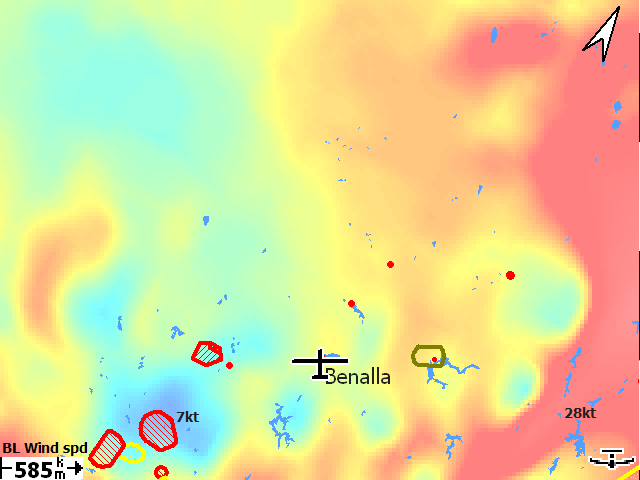
\includegraphics[angle=0,width=0.8\linewidth,keepaspectratio='true']{figures/rasp-blwindspd.png}
\end{center}

\item[H AS]
Maximale Höhe der Konvektionsschicht.

Für Blauthermik (''Trockenthermik'') ist dies die max.\ erreichbare Höhe eines Bartes.
Über flachem Gelände ist diese Höhe sogut wie nicht zu erreichen, da z.B.\ das
Eigensinken des Flugzeuges und andere Faktoren großen Einfluß haben.

Bei Wolkenthermik liegt die erreichbare Höhe über dieser Vorhersage, jedoch ist
bedingt durch die Wolkenbasis das Weitersteigen begrenzt.

Wenn Windscherungen auftreten, ist diese Vorhersage mit Vorsicht zu genießen,
da die Konvektionsschicht dann unkontrollierbar durchmischt wird und in praxi zu
anderen Ergebnissen führt.

\begin{center}
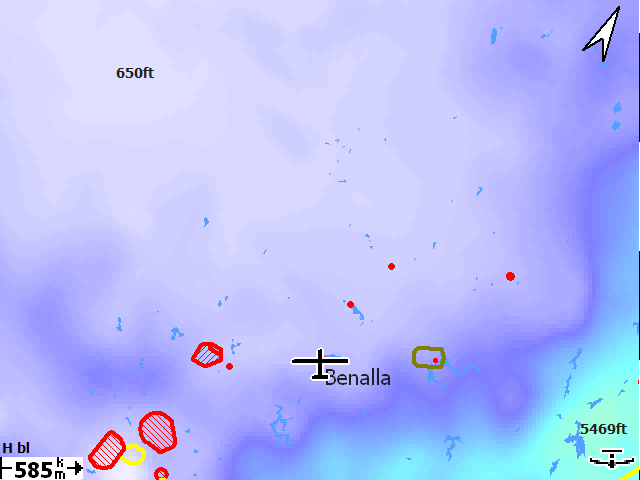
\includegraphics[angle=0,width=0.8\linewidth,keepaspectratio='true']{figures/rasp-hbl.png}
\end{center}

\item[dwcrit]
Max.\ Höhe über Grund der Blauthermik, bei der der Schnitt der Bärte  \textsl{unter} ca. 1,15$m/s$ liegt.

Diese Abschätzung liefert  wahrscheinlich eine bessere Verteilung der Thermikhöhe
der trockenen Luftmasse, als die max. Höhe der Konvektionsschicht - insbesondere, 
da die Ergebnisse der vertikalen Windscherungen anstelle der Thermik berücksichtigt
werden.


Beachte: Diese Abschätzungen neigen dazu, die max.\ Höhe der
nutzbaren trockenen Thermik eher zu unterschätzen.

Andererseits ist bei Wolken die max.\ Thermikhöhe durch  die Wolke an sich bis
zur Basis  beschränkt

Der evtl. feuchtadiabatische Weiteraufstieg des Luftpaketes ab Basishöhe wird bei
Blauthermik (trockene Luft) hier nicht berücksichtigt.

\item[KS Wolke]
Dieser Wert bietet eine zusätzliche Möglichkeit, die Wolkenbildung innerhalb der
Konvektionsschicht (KS) abzuschätzen und kann in Verbindung mit anderen
Wolkenvorhersageparametern vewendet werden.

Es wird eine sehr einfach Annahme zwischen Bedeckungsgrad und der maximalen
relativen Luftfeuchtigkeit der Konvektionsschicht getroffen.

Die Wolkenuntergrenze wird nicht vorhergesagt, ist aber unterhalb der
 KS-Obergrenze zu erwarten.


\begin{center}
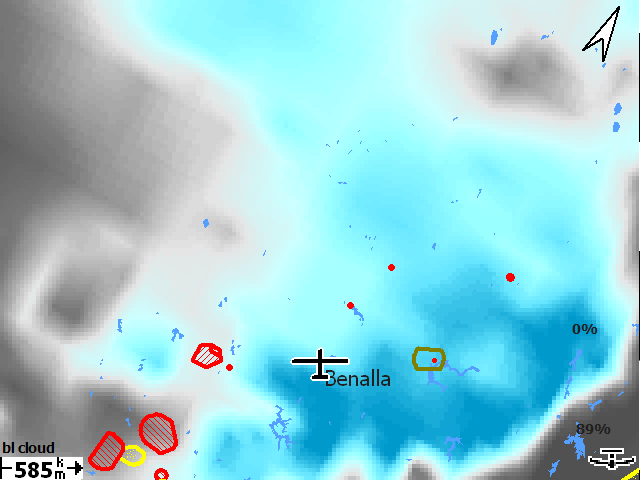
\includegraphics[angle=0,width=0.8\linewidth,keepaspectratio='true']{figures/rasp-blcloudpct.png}
\end{center}

\item[Sfc temp]

Temperatur in 2m Höhe über Grund.
Vergleicht man diese vorhergesagte Temperatur mit der tatsächlich gemessen Temperatur
erhält man ein grobes Maß  zur Abschätzung der Genauigkeit des Vorhersagemodelles.

Wenn die gemessene Temperatur signifikant unterhalb der vorhergesagten Temperatur
liegt, wird die Thermik sicher schlechter sein, als vorhergesagt.
\item[hwcrit]\todonum{wo ist der Unterschied zu dwcrit?}
Max.\ Höhe über Grund der Blauthermik, bei der der Schnitt der Bärte  \textsl{unter} ca. 1,15$m/s$ liegt.

Diese Abschätzung liefert  wahrscheinlich eine bessere Verteilung der Thermikhöhe
der trockenen Luftmasse, als die max. Höhe der Konvektionsschicht - insbesondere,
da die Ergebnisse der vertikalen Windscherungen anstelle der Thermik berücksichtigt
werden.

Beachte: Diese Abschätzungen neigen dazu, die max.\ Höhe der
nutzbaren trockenen Thermik eher zu unterschätzen.

Andererseits ist bei Wolken die max.\ Thermikhöhe durch  die Wolke an sich bis
zur Basis  beschränkt

Der evtl.\ feuchtadiabatische Weiteraufstieg des Luftpaketes ab Basishöhe wird bei
Blauthermik (trockene Luft) hier nicht berücksichtigt.
\item[blcwbase] Vorhergesagte Basis-Höhe von Cumulus-Wolken.

\item[wblmaxim] Maximale großflächige Auf-und Abbewegung der Konvektionsschicht, wie
z.B.\ bei Konvergenzen auftretend.

Positive Konvergenz (Aufsteigen der Schicht) ist mit Konvergenzlinien verbunden dargestellt.
Negative Konvergenz ''Divergenz'' ergibt eine absinkende Vertikalbewegung, was Inversion bedeutet.
Somit wird die Höhe der Thermik verringert bzw.\ begrenzt wird.
Absinkinversion -- kennt ja jeder\dots
\end{description}

\begin{maxipage}
Die Farbschemata welche für die RASP - Flächen benutzt werden, sind in der folgenden Tabelle wiedergegeben:

\begin{longtable}{c c c}
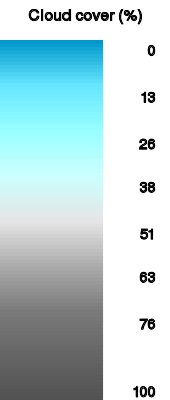
\includegraphics[angle=0,width=3cm,keepaspectratio='true']{figures/ramp-rasp-cloudpct.png}&
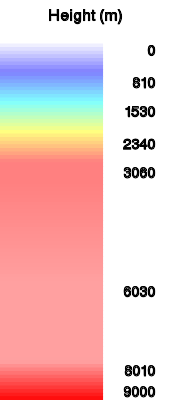
\includegraphics[angle=0,width=3cm,keepaspectratio='true']{figures/ramp-rasp-h.png}&
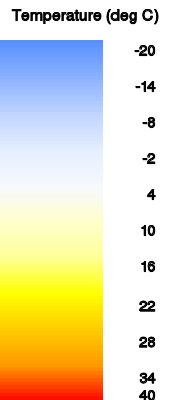
\includegraphics[angle=0,width=3cm,keepaspectratio='true']{figures/ramp-rasp-temperature.png}\\
\multicolumn{3}{c}{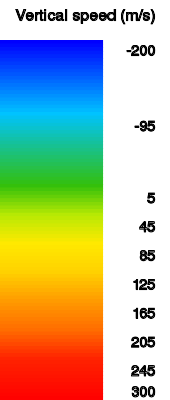
\includegraphics[angle=0,width=3cm,keepaspectratio='true']{figures/ramp-rasp-vertspeed.png}\quad
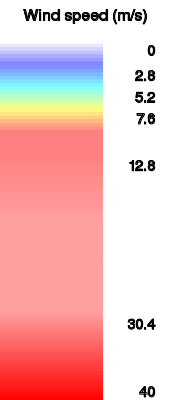
\includegraphics[angle=0,width=3cm,keepaspectratio='true']{figures/ramp-rasp-windspeed.png}} \\
\end{longtable}
\end{maxipage}
\todonum{Die Beschriftungen sollten unbedingt mal vereinheitlicht und angepasst werden.
Die Kurzformen bzw.\ Abküzungen sind extrem unübersichtlich. Was kann man hier wirklich gebrauchen 
und was ist nur Beiwerk?}